\section{Pianificazione}
Di seguito verranno presentate le tempistiche e le caratteristiche di
ciascun periodo. Al fine di mitigare i rischi derivanti da considerazioni
scorrette sulle tempistiche, sono stati inseriti oppurtuni slack.
\subsection{Analisi}
Questo periodo ha inizio il 2015-12-17 e termina il 2016-01-18, prima della data di consegna per la \textit{Revisione dei Requisiti}, in modo da poter contare su quattro giorni di \glossaryItem{Slack}, dunque la durata di questo periodo ammonta a trentadue giorni.

I ruoli attivi sono quelli di \textit{Amministratore}, \textit{Analista}, \textit{Responsabile}, \textit{Progettista} e \textit{Verificatore}.

La suddivisione in \glossaryItem{task} \`e incentrata sull'\textit{Analisi dei Requisiti}. Per tale motivo viene redatta e verificata prima di tutto la parte del \textit{Piano di \glossaryItem{progetto}} relativa all'\textit{Analisi}. Seguendo la prassi del modello incrementale, alla conclusione di ogni stesura segue un periodo di \glossaryItem{verifica}, per ottenere una \glossaryItem{Baseline} non corrotta.
\subsubsection{Diagramma di Gantt}
\begin{figure}[ht!]
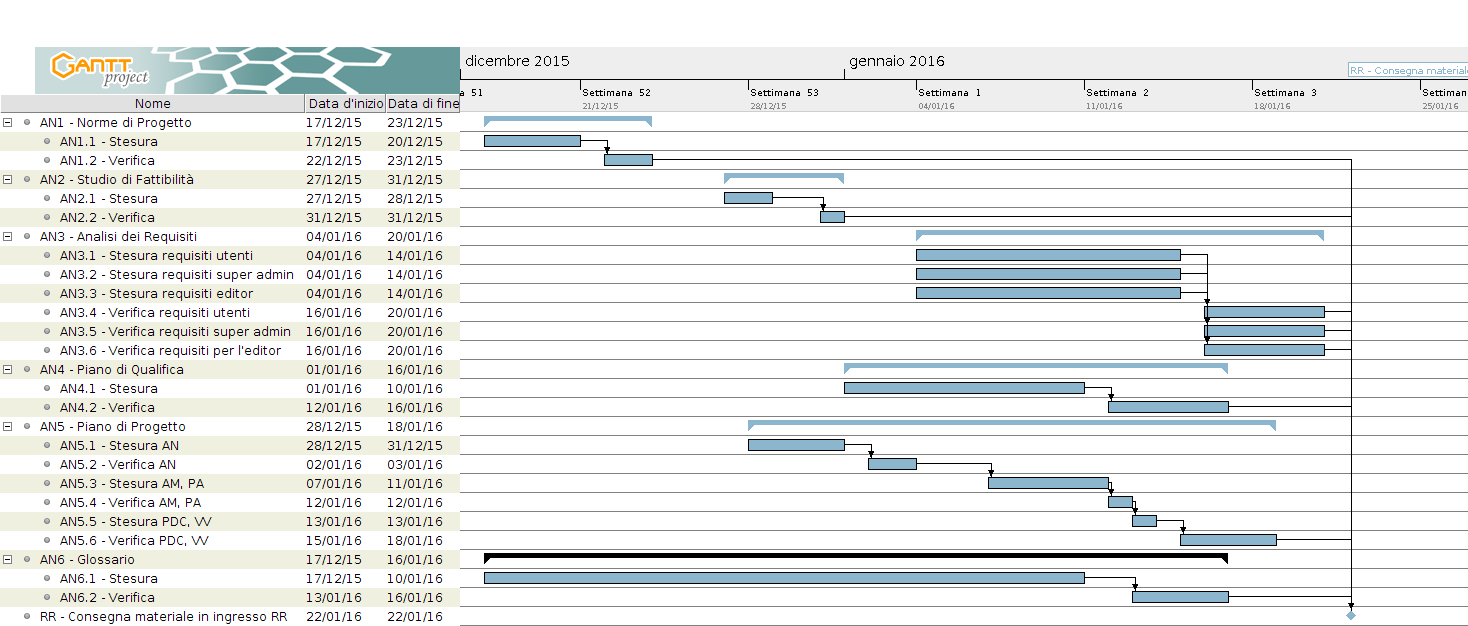
\includegraphics[width=1\textwidth]{res/img/pianificazione/Analisi.png}
\caption{Diagramma di Gantt, periodo di \textit{Analisi}}
\end{figure}

\subsubsection{Ripartizione ore}

\begin{table}[H]
	\centering
	\begin{tabular*}{1\textwidth}{ @{\extracolsep{\fill} } l l l c  }
	\hline
	\multicolumn{1}{c}{\textbf{Id}} & 
	\multicolumn{1}{c}{\textbf{Nome}} & 
	\multicolumn{1}{c}{\textbf{Ruolo}}& 
	\multicolumn{1}{c}{\textbf{Ore}} \\
	\hline
	
	\textbf{AN1} & \textbf{Norme di \glossaryItem{progetto}} \\
	\cline{3-4}
	AN1.1 & Stesura & Amministratore & 14\\ 
    & & Responsabile & 4 \\
    \cline{3-4}
	AN1.2 & \glossaryItem{Verifica} & Verificatore & 4\\
	
	\hline
	\textbf{AN2} & \textbf{Studio di Fattibilità} \\
	\cline{3-4}
	AN2.1 & Stesura & Analista & 6\\ 
    \cline{3-4}
	AN2.2 & \glossaryItem{Verifica} & Verificatore &  1\\
	
	\hline
	\textbf{AN3} & \textbf{Piano di \glossaryItem{progetto}} \\
	\cline{3-4}
	AN3.1 & Stesura AN & Amministratore & 2\\ 
    & & Responsabile & 16\\
    \cline{3-4}
	AN3.2 & \glossaryItem{Verifica} AN & Verificatore & 3\\
	\cline{3-4}
	AN3.3 & Stesura AM, PA & Amministratore & 8\\ 
    & & Responsabile & 10\\
	\cline{3-4}
	AN3.4 & \glossaryItem{Verifica} AM, PA & Verificatore & 2\\
	\cline{3-4}
	AN3.5 & Stesura PDC, VV & Amministratore & 4\\ 
        & & Responsabile & 3\\
	\cline{3-4}
	AN3.6 & \glossaryItem{Verifica} PDC, VV & Verificatore & 4\\
	

	\hline
	\textbf{AN4} & \textbf{Analisi dei Requisiti} \\
	\cline{3-4}
	AN4.1 & Stesura requisiti utenti & Analista & 16\\ 
    \cline{3-4}
	AN4.2 & Stesura requisiti \glossaryItem{super-admin} & Analista &  11\\
	\cline{3-4}
	AN4.3 & Stesure requisiti editor & Analista & 17\\ 
	\cline{3-4}
	AN4.4 & \glossaryItem{Verifica} requisiti utenti & Verificatore &  4\\
        \cline{3-4}
        AN4.5 & \glossaryItem{Verifica} requisiti \glossaryItem{super-admin} & Verificatore &  3\\
        \cline{3-4}
        AN4.6 & \glossaryItem{Verifica} requisiti per l'editor & Verificatore &  3\\
        \hline
        \textbf{AN5} & \textbf{Piano di qualifica} \\
	\cline{3-4}
	AN5.1 & Stesura & Progettista & 8\\
        & & Verificatore & 3\\
        \cline{3-4}
	AN5.2 & \glossaryItem{Verifica} & Verificatore & 6\\

        \hline
	\textbf{AN6} & \textbf{Glossario} \\
	\cline{3-4}
	AN6.1 & Stesura & Amministratore & 5\\
        \cline{3-4}
	AN6.2 & \glossaryItem{Verifica} & Verificatore & 3\\
	
	\hline
	\end{tabular*}
	\caption{Allocazione risorse, periodo di \textit{Analisi}}
	\end{table}

\newpage

\subsection{Analisi Miglioramenti}
Questo periodo ha inizio il 2016-02-17 e termina il 2016-02-26, a seguito dell'AR e prima dell'inizio stabilito del PA, per un totale di 9 giorni.


I ruoli attivi sono quelli di \textit{Amministratore}, \textit{Progettista}, \textit{Validatore}, \textit{Programmatore}, \textit{Responsabile}.


Lo scopo di questo periodo \`e il consolidamento, il miglioramento ed il cambiamento, se necessario, degli strumenti di supporto al \glossaryItem{progetto}, cercando di migliorare il pi\`u possibile l'ambiente di lavoro e i documenti seguendo la valutazione data dalla RR.\\
I membri del gruppo che occuperanno il ruolo di \textit{Amministratore} e \textit{Responsabile} saranno tenuti a ricercare strumenti alternativi ritenuti pi\`u validi rispetto a quelli adottati finora.\\
Il \textit{Validatore} dovr\`a occuparsi di verificare la \glossaryItem{qualit\`a} di quest'ultimi al fine di non incorrere, durante i periodi successivi, in prodotti non conformi ai livelli stabiliti dal \textit{Piano di Qualifica}, dovuti a cattiva strumentazione.\\
Infine il \textit{Programmatore}, affiancato dal \textit{Progettista}, avr\`a il compito di allestire l'ambiente di lavoro.

\subsubsection{Diagramma di Gantt}
\begin{figure}[ht!]
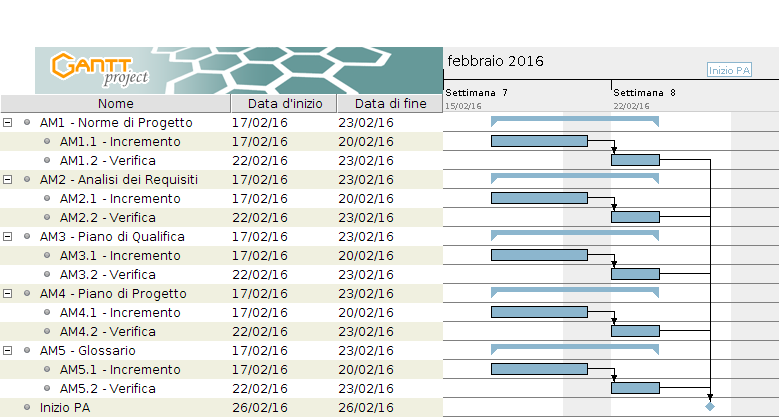
\includegraphics[width=1\textwidth]{res/img/pianificazione/AnalisiMiglioramenti.png}
\caption{Diagramma di Gantt, periodo di \textit{Analisi Miglioramenti}}
\end{figure}


\subsubsection{Ripartizione ore}

\begin{table}[H]
	\centering
	\begin{tabular*}{1\textwidth}{ @{\extracolsep{\fill} } l l l c  }
	\hline
	\multicolumn{1}{c}{\textbf{Id}} & 
	\multicolumn{1}{c}{\textbf{Nome}} & 
	\multicolumn{1}{c}{\textbf{Ruolo}}& 
	\multicolumn{1}{c}{\textbf{Ore}} \\
	\hline
	
	\textbf{AM1} & \textbf{Norme di \glossaryItem{progetto}} \\
	\cline{3-4}
	AM1.1 & \glossaryItem{Incremento} & Amministratore & 4\\ 
    \cline{3-4}
	AM1.2 & \glossaryItem{Verifica} & Verificatore & 2\\
	
	\hline
	\textbf{AM2} & \textbf{Analisi dei Requisiti} \\
	\cline{3-4}
	AM2.1 & \glossaryItem{Incremento} & Analista & 4\\ 
        \cline{3-4}
	AM2.2 & \glossaryItem{Verifica} & Verificatore & 2\\

        \hline
	\textbf{AM3} & \textbf{Piano di Qualifica} \\
	\cline{3-4}
	AM3.1 & \glossaryItem{Incremento} & Verificatore & 1\\
        & & Progettista & 3\\
        \cline{3-4}
	AM3.2 & \glossaryItem{Verifica} & Verificatore & 2\\
        
	\hline
	\textbf{AM4} & \textbf{Piano di \glossaryItem{Progetto}} \\
	\cline{3-4}
	AM4.1 & \glossaryItem{Incremento} & Responsabile & 1\\ 
        & & Amministratore & 3\\
    \cline{3-4}
	AM4.2 & \glossaryItem{Verifica} AN & Verificatore & 2\\

	\hline
	\textbf{AM5} & \textbf{Glossario} \\
	\cline{3-4}
	AM5.1 & \glossaryItem{Incremento} & Amministratore & 4\\ 
        \cline{3-4}
	AM5.2 & \glossaryItem{Verifica} & Verificatore & 2\\

        \hline
	\end{tabular*}
        \caption{Allocazione risorse, periodi di \textit{Analisi Miglioramenti}}
	\end{table}

\newpage

\subsection{Progettazione Architetturale}
Questo periodo ha inizio il 2016-02-27 e termina 2016-04-11, per un totale di 45 giorni.

I ruoli attivi sono quelli di \textit{Amministratore}, \textit{Analista}, \textit{Responsabile}, \textit{Progettista} e \textit{Verificatore}.

Si suddivide la \textit{Progettazione Architetturale} in progettazione dei requisiti fondamentali, desiderabili e opzionali. Inoltre, rimangono attive la stesura e la \glossaryItem{verifica} dei documenti scritti precedentemente, a causa di tutte le aggiunte e i miglioramenti emersi durante la \textit{Progettazione Architetturale}.

\subsubsection{Diagramma di Gantt}
\begin{figure}[ht!]
  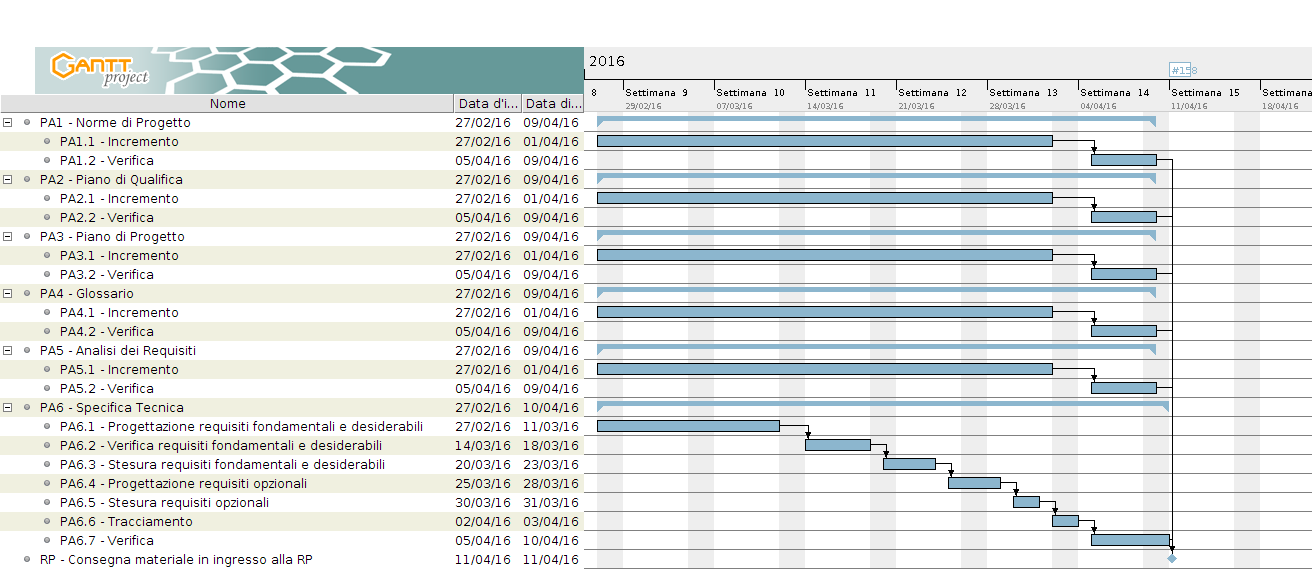
\includegraphics[width=1\textwidth]{res/img/pianificazione/ProgettazioneArchitetturale}
  \caption{Diagramma di Gantt, periodo \textit{Progettazione Architetturale}}
\end{figure}

\subsubsection{Ripartizione ore}
\begin{table}[H]
	\centering
	\begin{tabular*}{1\textwidth}{ @{\extracolsep{\fill} } l l l c  }
	\hline
	\multicolumn{1}{c}{\textbf{Id}} & 
	\multicolumn{1}{c}{\textbf{Nome}} & 
	\multicolumn{1}{c}{\textbf{Ruolo}}& 
	\multicolumn{1}{c}{\textbf{Ore}} \\
	\hline
	
	\textbf{PA1} & \textbf{Norme di \glossaryItem{progetto}} \\
	\cline{3-4}
	PA1.1 & \glossaryItem{Incremento} & Amministratore & 2\\ 
        \cline{3-4}
	PA1.2 & \glossaryItem{Verifica} & Verificatore & 1\\
	
	\hline
	\textbf{PA2} & \textbf{Piano di Qualifica} \\
	\cline{3-4}
	PA2.1 & \glossaryItem{Incremento} & Verificatore & 5\\ 
        & & Progettista & 2 \\
        \cline{3-4}
	PA2.2 & \glossaryItem{Verifica} & Verificatore &  3\\
	
	\hline
	\textbf{PA3} & \textbf{Piano di \glossaryItem{progetto}} \\
	\cline{3-4}
	PA3.1 & \glossaryItem{Incremento} & Responsabile & 2\\ 
        \cline{3-4}
	PA3.2 & \glossaryItem{Verifica} & Verificatore & 1\\

	\hline
	\textbf{PA4} & \textbf{Glossario} \\
	\cline{3-4}
	PA4.1 & \glossaryItem{Incremento} & Amministratore & 6\\ 
        \cline{3-4}
	PA4.2 & \glossaryItem{Verifica} & Verificatore & 4\\

        \hline
        \textbf{PA5} & \textbf{Analisi Requisiti}\\
        \cline{3-4}
        PA5.1 & \glossaryItem{Incremento} & Analista & 3\\
        \cline{3-4}
        PA5.2 & \glossaryItem{Verifica} & Verificatore & 4\\

        \hline
        \textbf{PA6} & \textbf{Specifica Tecnica} \\
	\cline{3-4}
	PA6.1 & Progettazione requisiti fondamentali e desiderabili & Progettista & 57\\ 
        \cline{3-4}
	PA6.2 & \glossaryItem{Verifica} requisiti fondamentali e desiderabili & Verificatore & 26\\
        \cline{3-4}
	PA6.3 & Stesura requisiti fondamentali e desiderabili & Progettista & 17\\
        \cline{3-4}
	PA6.4 & Progettazione requisiti opzionali & Progettista & 35\\

        \hline
	PA6.5 & Stesura requisiti opzionali & Progettista & 10\\
        \cline{3-4}
	PA6.6 & \glossaryItem{Tracciamento} & Progettista & 20\\
        \cline{3-4}
	PA6.7 & \glossaryItem{Verifica} & Verificatore & 30\\
        \hline
	\end{tabular*}
        \caption{Allocazione risorse, periodo di \textit{Progettazione Architetturale}}
	\end{table}

\newpage

\subsection{Progettazione di Dettaglio e Codifica}
Questo periodo ha inizio il 2016-04-19 e termina il 2016-05-14, per un totale 30 giorni.

I ruoli attivi in questo periodo sono quello di \textit{Amministratore}, \textit{Progettista}, \textit{Programmatore}, \textit{Responsabile} e \textit{Verificatore}.

Oltre agli \glossaryItem{incrementi} presenti per mantenere aggiornati i documenti, in questo periodo si pianifica la realizzazione del prodotto completo che soddisfi i requisiti fondamentali, desiderabili ed opzionali. Una volta avvenuta la \glossaryItem{verifica} su tutta la progettazione, si effettuano la codifica e la stesura del manuale dell'utente, da consegnare al proponente come \glossaryItem{verifica} dei requisiti richiesti e della \glossaryItem{qualit\`a} fissata.

\subsubsection{Diagramma di Gantt}
\begin{figure}[ht!]
  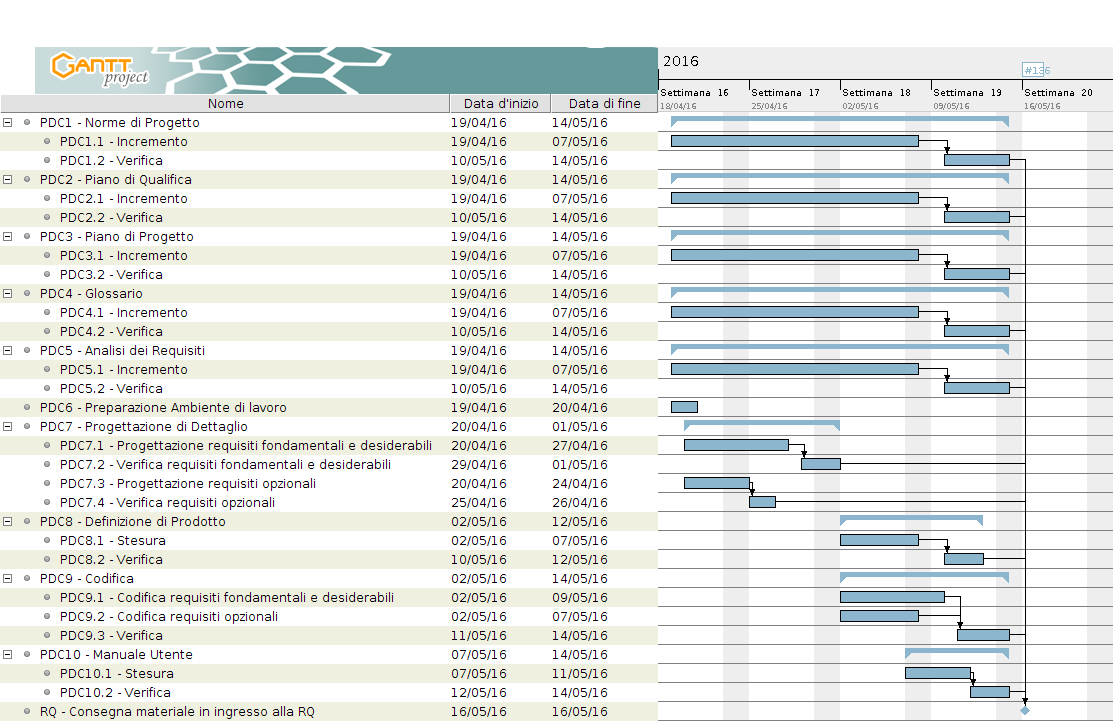
\includegraphics[width=1\textwidth]{res/img/pianificazione/ProgettazioneDettaglioECodifica.png}
  \caption{Diagramma di Gantt, periodo \textit{Progettazione di Dettaglio e Codifica}}
\end{figure}

\subsubsection{Ripartizione orario}
\begin{table}[H]
	\centering
	\begin{tabular*}{1\textwidth}{ @{\extracolsep{\fill} } l l l c  }
	\hline
	\multicolumn{1}{c}{\textbf{Id}} & 
	\multicolumn{1}{c}{\textbf{Nome}} & 
	\multicolumn{1}{c}{\textbf{Ruolo}}& 
	\multicolumn{1}{c}{\textbf{Ore}} \\
	\hline
	
	\textbf{PDC1} & \textbf{Norme di \glossaryItem{Progetto}} \\
	\cline{3-4}
	PA1.1 & \glossaryItem{Incremento} & Amministratore & 3\\ 
        \cline{3-4}
	PDC1.2 & \glossaryItem{Verifica} & Verificatore & 1\\
	
	\hline
	\textbf{PDC2} & \textbf{Piano di Qualifica} \\
	\cline{3-4}
	PDC2.1 & \glossaryItem{Incremento} & Progettista & 4\\
        & & Verificatore & 2\\
        \cline{3-4}
	PDC2.2 & \glossaryItem{Verifica} & Verificatore & 2\\
	
	\hline
	\textbf{PDC3}  & \textbf{Piano di \glossaryItem{progetto}} \\
	\cline{3-4}
	PDC3.1 & \glossaryItem{Incremento} & Responsabile & 3\\ 
        \cline{3-4}
	PDC3.2 & \glossaryItem{Verifica} & Verificatore & 2\\

	\hline
	\textbf{PDC4} & \textbf{Glossario} \\
	\cline{3-4}
	PDC4.1 & \glossaryItem{Incremento} & Amministratore & 3\\ 
        \cline{3-4}
	PDC4.2 & \glossaryItem{Verifica} & Verificatore & 1\\

        \hline
        \textbf{PDC5} & \textbf{Analisi dei Requisiti}\\
        \cline{3-4}
        PDC5.1 & \glossaryItem{Incremento} & Analista & 3\\
        \cline{3-4}
        PDC5.2 & \glossaryItem{Verifica} & Verificatore & 2\\

        \hline
        \textbf{PDC6} & \textbf{Preparazione Ambiente di lavoro} & Amministratore & 10\\

        \hline
        \textbf{PDC7} & \textbf{Progettazione di Dettaglio} \\
	\cline{3-4}
	PDC5.1 & Progettazione requisiti fondamentali e desiderabili & Progettista & 48\\ 
        \cline{3-4}
	PDC5.2 & \glossaryItem{Verifica} requisiti fondamentali e desiderabili & Verificatore & 10\\
        \cline{3-4}
	PDC5.3 & Progettazione requisiti opzionali & Progettista & 28\\
        \cline{3-4}
	PDC5.4 & \glossaryItem{Verifica} requisiti opzionali & Verificatore & 5\\

        \hline
        \textbf{PDC7} & \textbf{Definizione di Prodotto} \\
	\cline{3-4}
	PDC7.1 & Stesura & Progettista & 40\\ 
        \cline{3-4}
        PDC7.2 & \glossaryItem{Verifica} & Verificatore & 11\\

        \hline
        \textbf{PDC8} & \textbf{Codifica} \\
	\cline{3-4}
	PDC8.1 & Codifica requisiti fondamentali e desiderabili & \glossaryItem{Programmatore} & 85\\
        \cline{3-4}
	PDC8.2 & Codifica requisiti opzionali & \glossaryItem{Programmatore} & 56\\
        \cline{3-4}
        PDC8.3 & \glossaryItem{Verifica} & Verificatore & 9\\
        \hline
	\textbf{PDC8} & \textbf{Manuale Utente} \\
	\cline{3-4}
	PDC8.1 & Stesura & Amministratore & 34\\ 
        \cline{3-4}
	PDC8.2 & \glossaryItem{Verifica} & Verificatore & 9\\
        \hline
	\end{tabular*}
        \caption{Allocazione risorse, periodo di \textit{Progettazione di Dettaglio e Codifica}}
\end{table}

\newpage

\subsection{Validazione}
Questo periodo ha inizio il 2016-05-24 e termina il 2016-06-09, per un totale di 16 giorni.
I ruoli attivi sono quello di \textit{Amministratore}, \textit{Progettista}, \textit{Responsabile}, \textit{Verificatore}.

Con l'adozione del modello incrementale il risultato \`e un ultimo momento molto breve in cui eseguire i test di sistema e rilasciare il prodotto completo per il collaudo della \textit{Revisione di Accettazione}. Nello stesso momento vengono redatte le ultime \glossaryItem{versioni} dei documenti da rilasciare alla commissione e al \glossaryItem{committente}.

\subsubsection{Diagramma di Gantt}
\begin{figure}[ht!]
  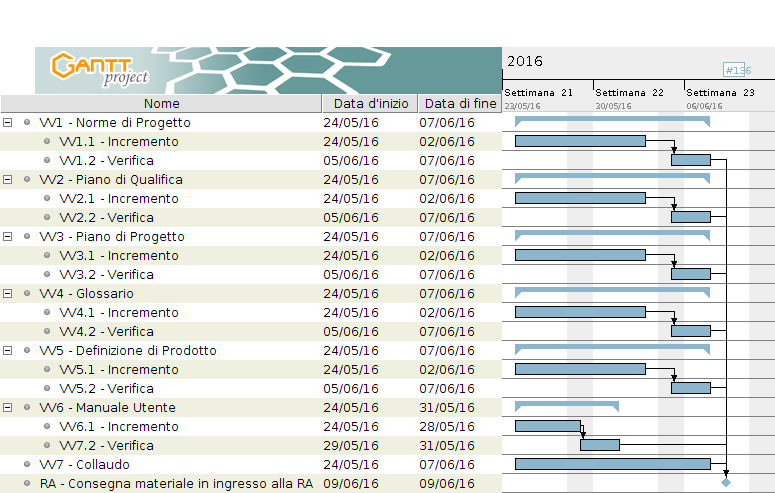
\includegraphics[width=1\textwidth]{res/img/pianificazione/VerificaEValidazione.png}
  \caption{Diagramma di Gantt, periodo di \textit{Validazione}}
\end{figure}

\subsubsection{Ripartizione orario}

\begin{table}[H]
	\centering
	\begin{tabular*}{1\textwidth}{ @{\extracolsep{\fill} } l l l c  }
	\hline
	\multicolumn{1}{c}{\textbf{Id}} & 
	\multicolumn{1}{c}{\textbf{Nome}} & 
	\multicolumn{1}{c}{\textbf{Ruolo}}& 
	\multicolumn{1}{c}{\textbf{Ore}} \\
	\hline
	
	\textbf{VV1} & \textbf{Norme di \glossaryItem{progetto}} \\
	\cline{3-4}
	VV1.1 & \glossaryItem{Incremento} & Amministratore & 2\\ 
    \cline{3-4}
	VV1.2 & \glossaryItem{Verifica} & Verificatore & 2\\
	
	\hline
	\textbf{VV2} & \textbf{Piano di Qualifica} \\
	\cline{3-4}
	VV2.1 & \glossaryItem{Incremento} & Verificatore & 2\\
        \cline{3-4}
	VV2.2 & \glossaryItem{Verifica} & Verificatore & 2\\
	
	\hline
	\textbf{VV3} & \textbf{Piano di \glossaryItem{progetto}} \\
	\cline{3-4}
	VV3.1 & \glossaryItem{Incremento} & Responsabile & 6\\
        \cline{3-4}
	VV3.2 & \glossaryItem{Verifica} & Verificatore & 2\\

	\hline
	\textbf{VV4} & \textbf{Glossario} \\
	\cline{3-4}
	VV4.1 & \glossaryItem{Incremento} & Amministratore & 1\\
    \cline{3-4}
	VV4.2 & \glossaryItem{Verifica} & Verificatore & 2\\

        \hline
        \textbf{VV5} & \textbf{Definizione di Prodotto} \\
	\cline{3-4}
        VV5.1 & \glossaryItem{Incremento} & Progettista & 12\\
        \cline{3-4}
	VV5.2 & \glossaryItem{Verifica} & Verificatore & 5\\

        \hline
        \textbf{VV6} & \textbf{Manuale Utente} \\
	\cline{3-4}
        VV5.1 & \glossaryItem{Incremento} & Amministratore & 10\\
        \cline{3-4}
	VV5.2 & \glossaryItem{Verifica} & Verificatore & 8\\
                
        \hline
        \textbf{VV7} & \textbf{Collaudo} & Verificatore & 47\\
        & & \glossaryItem{Programmatore} & 5\\

        \hline
	\end{tabular*}
        \caption{Allocazione risorse, periodo di \textit{Validazione}}
	\end{table}
\newpage
